% \newpage
\section{Method}

This section introduces our novel Local-Alignment Contrastive (LAC) loss function employed within our framework where video alignment serves as the pretext task, as visualized in Fig. \ref{fig: vis_method}. Specifically, we will derive the forward and backward passes of the differentiable local alignment loss and explain how we ensure consistency within our method.

\subsection{Notations} \label{sec: 3_notation}

Let $V^1$ and $V^2$ represent a pair of video frames. 
Following \cite{2022_carl}, we preprocess the frames via temporal random cropping to generate two cropped videos, each consisting of $T$ frames.
We denote these cropped videos as $(V^1, S^1)$ and $(V^2, S^2)$, where $S \in \mathbb{R}^T$ contains the indices of the sampled frames. 
Next, we apply augmentations, resulting in $\widetilde{V}^1$ and $\widetilde{V}^2$. 
Finally, these frames are processed through an encoder to obtain embeddings $Z^1$ and $Z^2$.
Each embedding $Z \in \mathbb{R}^{T \times E}$ represents a sequence with length $T$ and embedding dimension $E$.
The objective is to train the encoder so that frames from $V^1$ and $V^2$ depicting the same action have minimized distances between the corresponding embeddings.

\begin{figure}[t]
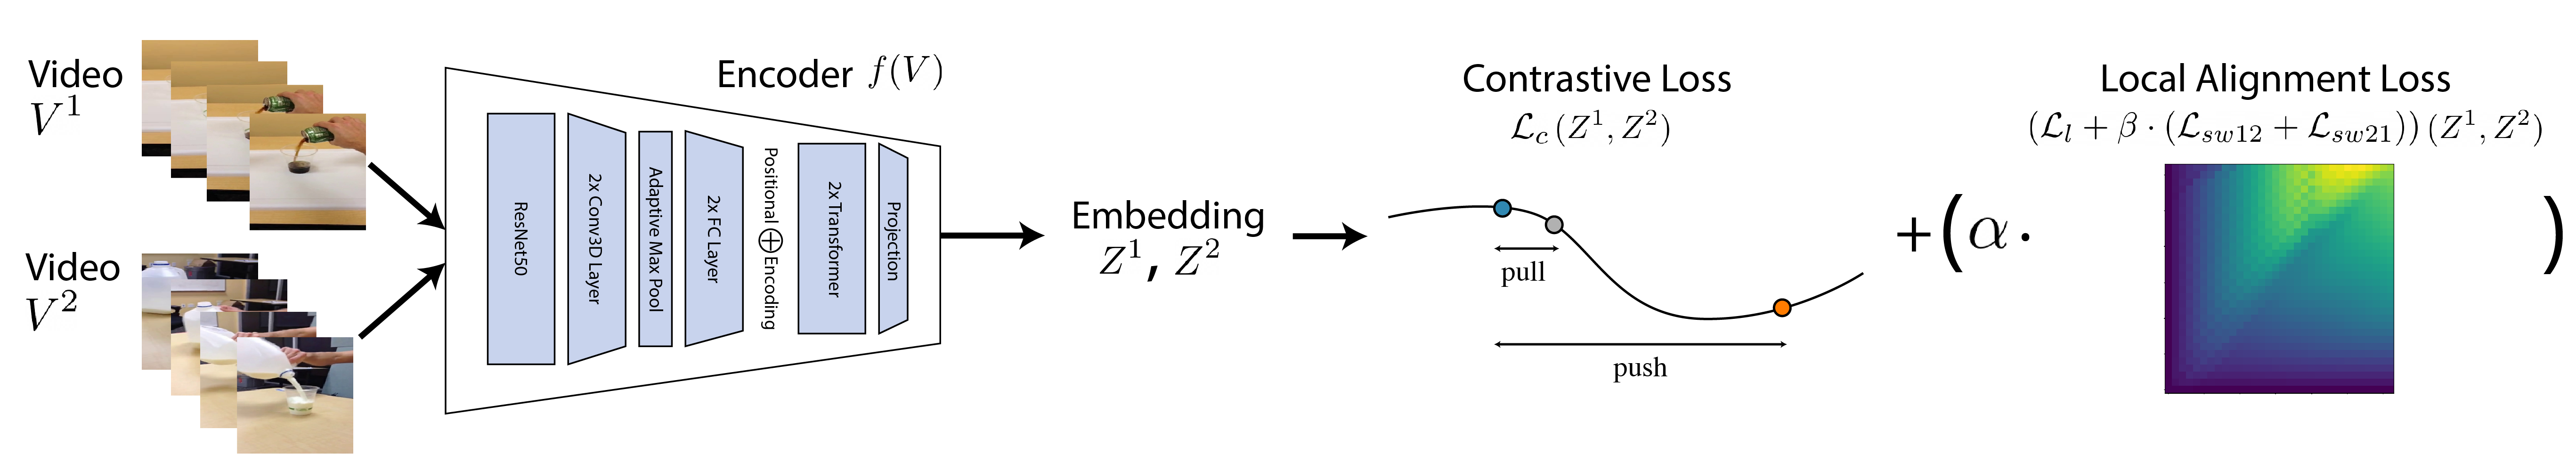
\includegraphics[width=1\textwidth]{images/a2.png}
\caption{Our framework uses Local Alignment Loss and Contrastive Loss to optimize embeddings generated by an encoder that processes input videos after they have undergone spatio-temporal data augmentation.}
\label{fig: vis_method}
\end{figure}
\subsection{Background}

Prior approaches \cite{2021_lav, 2021_gta} use DTW as the principal method for temporal alignment loss. Given a cost matrix $d_{i, j}$ that measures the cost of matching elements between embeddings $Z^1$ and $Z^2$, DTW seeks the optimal path that minimizes this cost. The feasible paths must satisfy constraints of matching endpoints, monotonicity, and continuity. Initially, the computational complexity of DTW grows exponentially with the length of the sequences due to the combinatorial explosion of possible alignment paths. However, by using dynamic programming, DTW's complexity reduced to polynomial time. The DTW algorithm can be formulated as follows:

\begin{equation}
    D_{i, j} = d_{i, j} + \min \left\{
    \begin{array}{l}
         D_{i-1, j-1} \\
         D_{i-1, j} \\
         D_{i, j-1} \\
    \end{array}
    \right.
    \label{eq: dtw}
\end{equation}

where $D_{i, j}$ represents the cumulative distance up to the point $(i, j)$ in the cost matrix, and $d_{i, j}$ denotes the local distance between elements $Z^1_i$ and $Z^2_j$. The non-differentiable nature of the $\min$ operator in the DTW formulation presents challenges for gradient-based optimization techniques. To address this, prior methods \cite{2021_lav, 2021_gta} utilize Soft-DTW \cite{2017_softdtw}, which replaces the discrete $\min$ operator with a differentiable/smoothed version denoted as $\min^\gamma$. As the parameter $\gamma$ approaches zero, he behavior of $\min^\gamma$ approximates that of the discrete $\min$ operator. This substitution enables the use of gradient-based optimization in DTW while preserving its alignment capabilities.

\subsection{Differentiable Local-Alignment} \label{sec: 3_diffla}

Despite the advantages offered by Soft-DTW \cite{2017_softdtw}, it inherently maintains the global alignment characteristic, ensuring continuity throughout the sequence. This attribute of global alignment may prove suboptimal in scenarios where localized alignment strategies, such as those implemented by the SW algorithm \cite{1981_sw}, are preferable. The SW algorithm \cite{1981_sw} supports localized matching, providing enhanced flexibility and increased sensitivity to similarities within subsequences. In response, we propose a differentiable SW local-alignment approach as our method for temporal alignment loss.

We consider a pair of embeddings, $(Z^1, S^1)$ and $(Z^2, S^2)$, with corresponding sampled indices, tasked with determining the optimal alignment between these embeddings.
We begin by calculating a similarity matrix, $S \in \mathbb{R}^{T \times T}$, using the inverted Euclidean distance to yield higher values that indicate increased similarity between the points in $Z^1$ and $Z^2$. 
Utilizing dynamic programming, the SW algorithm effectively determines the optimal alignment by maximizing a score derived from pairwise similarities within the matrix. 
The alignment algorithm can be formally expressed as follows:


\begin{equation}
    D_{i,j} = S_{i, j} + \max \left\{
    \begin{array}{l}
        0 \\
        D_{i - 1,j - 1} \\
        I_{x_{i - 1,j - 1}} \\
        I_{y_{i - 1,j - 1}}
    \end{array} \label{eq: la_D}
\right. \\
\end{equation}

\begin{equation}
I_{x_{i,j}} = \max \left\{
    \begin{array}{l}
        D_{i, j - 1} - g_{o_{i, j}} \\
        I_{x_{i, j -1}} - g_{e_{i, j}}
    \end{array}
\right. \label{eq: la_Ix}
\end{equation}

\begin{equation}
I_{y_{i,j}} = \max \left\{
    \begin{array}{l}
        D_{i - 1, j} - g_{o_{i, j}}  \\
        I_{x_{i - 1, j}} - g_{o_{i, j}} \\
        I_{y_{i - 1, j}} - g_{e_{i, j}} 
    \end{array}
\right. \label{eq: la_Iy}
\end{equation}

where the initial values are set to $D(i, 0) = D(0, j) = I_x(i, 0) = I_x(0, j) = I_y(i, 0) = I_y(0, j) = -\infty$ for all indices $i, j = 1, \ldots, T$. The matrix $D$ described in Eq. \ref{eq: la_D} acts as the primary scoring matrix, representing the cumulative maximum score at each matrix coordinate $(i, j)$. The matrices $I_x$ and $I_y$ detailed in Eq. \ref{eq: la_Ix} and Eq. \ref{eq: la_Iy}, represent the scores associated with introducing gaps along the $x$ and $y$ axes. Additionally, $g_o$ and $g_e$ are used to specify the penalties for opening and extending gaps.

Similar to Soft-DTW \cite{2017_softdtw}, our differentiable temporal alignment loss function uses a smoothed version of the discrete $\max$ function, denoted as $\max^\gamma$. This smooth approximation is formally defined as:

\begin{equation}
  \max{}^{\gamma}(u_1, \ldots, u_n) := \gamma \, \log \, \sum_{i=1}^{n} \, e^{u_i/\gamma}  \label{eq: smooth_max}
\end{equation}

where $\gamma > 0$ is a smoothing parameter that controls the approximation's fidelity to the original $\max$ function. As $\gamma$ approaches zero, the smoothed $\max^\gamma$ function increasingly approximates the behavior of the standard $\max$ function, enabling a differentiable formulation that can be integrated into gradient-based optimization frameworks. The gradient of the smoothed $\max^\gamma$ with respect to each input $u_i$ is calculated as follows:

\begin{align}
    \frac{\partial \max{}^\gamma(\{u_1,\ldots, u_n\})}{\partial u_i} & = \exp\left(\frac{u_i - \max{}^\gamma(\{u_1,\ldots,u_n\})}{\gamma}\right)
    \label{eq: partial_softmax}
\end{align}

This expression aligns with the softmax function. 
By differentiating the smoothed maximum score with respect to each input, our model directly utilizes derivative-sensitive parameters such as the similarity score ($S$), gap open penalty ($g^o$), and gap extend penalty ($g^e$). 
As a result, we define our differentiable local alignment loss as \(\mathcal{L}_{sw_{ij}} = \text{SW}(\text{sim}(Z^i, Z^j))\).
The ($\text{sim}$) function calculates the similarity between two embeddings and generates a similarity matrix $S$. 
Unlike prior differentiable SW implementations \cite{2023_sw1, 2023_sw2} that depend on supervised learning, our approach integrates the differentiable SW algorithm within a self-supervised framework.

\subsection{Final Loss} \label{sec: 3_total}

Following the approach in \cite{2022_carl}, our contrastive loss is modeled after the NT-Xent loss from SimCLR \cite{2020_simclr}. 
This loss function calculates absolute pairwise distances between embeddings $(Z^1, S^1)$ and $(Z^2, S^2)$,  subsequently forming a Gaussian-weighted positive label distribution.
This distribution is then contrasted against normalized similarity logits using the Kullback-Leibler divergence. 
The contrastive loss is mathematically expressed as:

\begin{equation}
    \mathcal{L}_c = - \frac{1}{T} \sum_{i, j=1}^T \left( \frac{G(s_i^1 - s_j^2)}{\sum_{k=1}^T G(s_i^1 - s_k^2)} \log \frac{\exp(\text{sim}(z_i^1, z_j^2) / \tau)}{\sum_{k=1}^T \exp(\text{sim}(z_i^1, z_k^2) / \tau)} \right)
\end{equation}

where $\tau$ represents the temperature parameter, $G$ denotes the Gaussian weighting function applied to the absolute pairwise distances, and $(\text{sim})$ measures the normalized similarity between embeddings.
To ensure consistency between contrastive and local alignment losses, we synchronize our temporal local loss by utilizing the primary score matrix $D_{12}$ and $D_{21}$ from $\mathcal{L}_{sw12}$ and $\mathcal{L}_{sw21}$.
Following the application of the softmax function to $D$, the resulting matrix is referred to as $\Tilde{D}$.
The logits matrix \(L\) is then derived by performing an element-wise multiplication of \(\Tilde{D}_{12}\) and \(\Tilde{D}_{21}^T\). 
The cross-entropy loss for this logits matrix against the Gaussian-weighted labels is calculated as follows:


\begin{align*}
\mathcal{L}_l &= -\frac{1}{T} \sum_{i, j=1}^T  \left(\, \frac{G(s_i^1 - s_j^2)}{\sum_{k=1}^T G(s_i^1 - s_k^2)} \log \left( \frac{\exp(\text{L}_{ij})}{\sum_{k=1}^T \exp^(\text{L}_{ik})} \right) \right), \\
\text{where} 
\,\ \Tilde{D}_{12, ij} & = \frac{\exp(D_{12, ij}/\tau)}{\sum_{k=1}^T \exp(D_{12, ik}/\tau)} \,,
\,\ \Tilde{D}_{21, ij} = \frac{\exp(D_{21, ij}/\tau)}{\sum_{k=1}^T \exp(D_{21, ik}/\tau)} \,,
\,\ L = \Tilde{D}_{12} \cdot \Tilde{D}_{21}^T
\end{align*}

Our proposed loss function, referred as Local-Alignment Contrastive (LAC), integrates contrastive and local alignment losses. It is formally defined as follows:

\begin{equation}
    \mathcal{L} = \mathcal{L}_c + \alpha \cdot (\mathcal{L}_l + \beta \cdot (\mathcal{L}_{sw12} + \mathcal{L}_{sw21}))
\end{equation}

where \(\alpha\) and \(\beta\) are weights used to balance the components of the loss, set to 0.01 and 1, respectively.

